\section{Architektur}
\label{sec:komponenten:architektur}

Die in dieser Arbeit zugrunde liegende Architektur folgt dem Ansatz von\cite{Truyen2016}, in dem eine Containerbasierte
Architektur für \ac{SaaS} Anwendungen vorgestellt wird. Kubernetes spielt hierbei eine wichtige Rolle. Es dient dem State
Managment, der Isolation der Workloads sowie der Authentifizierung für Tenants. Hierbei ist jede Komponente des \ac{SaaS}
mit Kubernetes integriert.

\begin{figure}[h]
  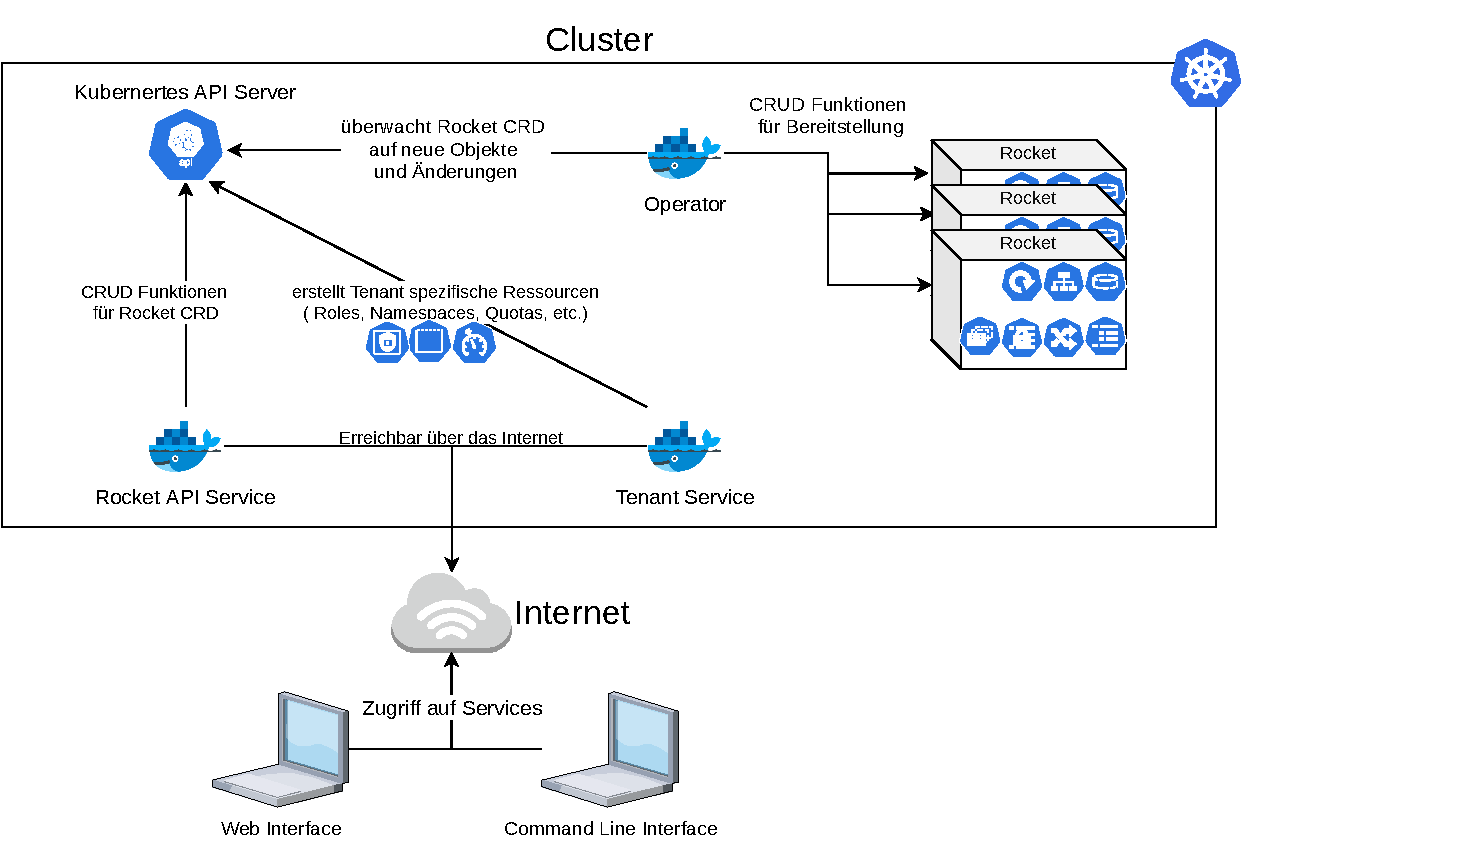
\includegraphics[width=45em]{gfx/chapters/3_komponenten/saas_architecture.pdf}
  \caption{Architektur des \ac{SaaS}}
  \label{fig:architektur}
\end{figure}

In \ref{fig:architektur} wird die Architektur bildlich dargestellt.
Hier erkennt man, dass die Hauptkomponenten der Serverseite alle mit der Kubernetes API kommunizieren,
um den gewünschten State des Clients zu erzielen. Der Operator \ref{sec:komponenten:operator} dient als Komponente zum tatsächlichen
Erstellen der Rocket und MongoDB\footnote{Dokumentenorientierte NoSQL-Datenbank \href{https://www.mongodb.com/}{MongoDB}}
Container sowie Netzwerk-, Anwendungs- und Speicherkonfiguration.
Bei einer Änderung der Spezifikation eines Rocket Objekts, wird automatisch eine Synchronisation des 
Clusters vorgenommen, sodass die gewünschte Konfiguration im Cluster deployed ist.
% TODO: Include Ref to CRD Chapter

Der Rocket API Service \ref{sec:komponenten:rocket-api-service} hat die Aufgabe, 
dass vom Operator definierte \ac{CR} im Kubernetes Cluster zu erstellen, während der 
Tenant Service \ref{sec:komponenten:tenant-service} sich um die Konfiguration des Users im Cluster kümmert.
Hierbei werden Objekte wie beispielsweise Rollen, Namespaces und Quotas erstellt.

Clients \ref{sec:komponenten:clients} haben die Rolle, mit dem Nutzer zu interagieren. Hierbei kann jegliche Art genutzt werden,
zum Beispiel ein \emph{\ac{CLI}} Tool\footnote{Programm zur Interaktion mit dem User via Kommandozeile}
, \emph{\ac{IaC} Tools} oder ein \emph{Web Interface}. Aus Zeitgründen wurde für die Referenzimplementation nur
ein \ac{CLI} Client implementiert.
